\section{Examples}
Throughout the paper, two examples will be used. The first is the \emph{banana} distribution, which is a 2d Gaussian, which has been squeezed into a half-moon shape as depicted in figure \ref{fig:banana_distr_contour}:
$$
p(x,y) = \frac{1}{2\pi \sigma_x \sigma_y} \exp\left(-\frac{1}{2}(x/\sigma_x)^2 + (y-c\cdot x^2)^2/\sigma_y^2\right)
$$
where $c$ is a curvature constant that controls the squeeziness.

The second example is a regression problem using a small neural network as a function approximator. The model takes a one-dimensional input and output, has two hidden layers of each 10 neurons, and uses ReLU activation function. The network has been randomly initialized, 50 training data samples has been generated with  $\sigma_t=0.05$ sampling noise and finally, the model has been fine-tuned to fit to the sampled data (to guarantee that the parameters actually reflects a minimum in the loss landscape with respect to the training data). What we want to see here is a model that is certain about the mean value in the areas where there are data points, but expresses higher uncertainty in the interval $[-0.5, 0.5]$ where there is no training data available.

\begin{figure}[h]
    \centering
    \subfloat[Banana probability density with $c=0.2$, $\sigma_x=2$, and $\sigma_y=.5$]{
        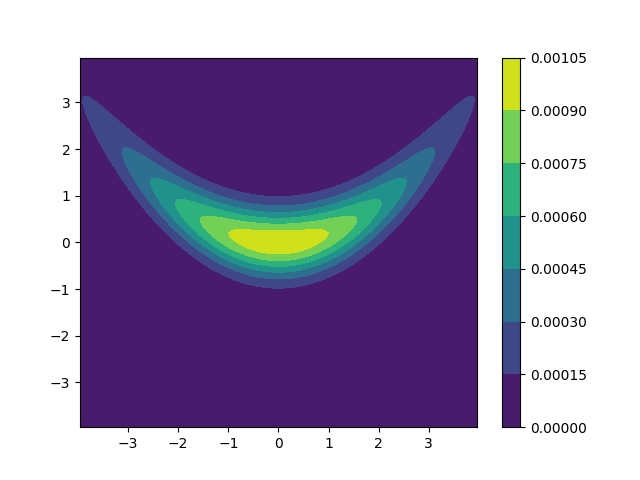
\includegraphics[width=.45\linewidth]{report/figures/banana_distr_contour.png}
        \label{fig:banana_distr_contour}
    }
    \hfill
    \subfloat[Function approximator]{
        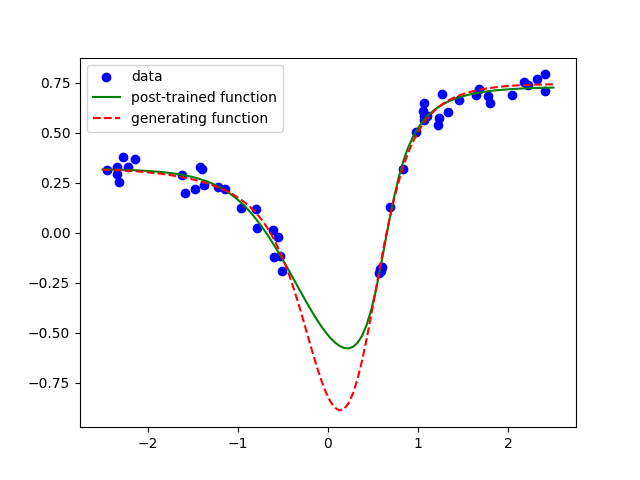
\includegraphics[width=.45\linewidth]{report/figures/post_trained_function.png}
        \label{fig:post_trained_function}
    }
    \caption{Examples used in this paper}
    \label{fig:examples_figs}
\end{figure}